\section{Analisi}
\subsection{Requisiti}

Il gruppo si pone come obiettivo quello di realizzare la trasposizione videoludica del gioco da tavolo Carcassonne. Si tratta di un gioco da 2 a 6 giocatori dove ognuno deve posizionare delle tessere e dei seguaci, o pedine, con lo scopo di realizzare punti. Chi alla fine della partita avrà totalizzato più punti verrà proclamato vincitore.

\subsection*{Requisiti funzionali}
Il gioco dovrà permettere ai giocatori che ne partecipano, ognuno identificato univocamente da nome e colore, di piazzare e ruotare tessere ed eventualmente posizionarvi sopra un seguace. E' necessario:

\begin{itemize}
\item Permettere il posizionamento delle tessere solo se posizionate in modo adiacente alle tessere già in campo ed esclusivamente nel caso in cui ogni lato della tessera corrente combaci con il lato della tessera vicina
\item Permettere il posizionamento di seguaci su strutture appartenenti alla tessera appena piazzata e senza altri seguaci
\item Calcolare il punteggio dei giocatori, sia nel momento in cui viene chiusa una struttura, che alla fine della partita
\item Permettere la navigazione del campo di gioco
\item Permettere di scartare una tessera che non possa essere piazzata in nessuna delle posizioni libere
\item Permettere la selezione del numero dei giocatori e assegnare un nome ed un colore ad ognuno
\item Gestire l'ampliamento e l'unione di praterie, città e strade
\end{itemize}

\subsection*{Requisiti non funzionali}
\begin{itemize}
\item Menù di pausa
\item Visualizzazione grafica e dinamica dei seguaci rimanenti 
\item Pannello per la scelta del colore del giocatore
\item Decorazioni, sfondi e distanziamento fra i vari componenti grafici
\item Supporto di espandibilità futura per l'implementazione di immagini di profilo dei giocatori
\item Supporto alla lingua italiana e inglese
\item Supporto per partecipare alla stessa partita da più interfacce
\item Supporto per future espansioni con l'aggiunta di nuove tessere e seguaci
\end{itemize}

\subsection{Analisi e modello del dominio}
L'analisi e il modello di dominio di Caesena possono essere suddivisi in diversi componenti chiave: le tessere, i seguaci e il sistema di punteggio.

Le tessere, estratte casualmente, devono essere poste in maniera adiacente in modo che combacino tra di loro e formino strutture, ovvero strade, praterie, città e monasteri. Posizionando un seguace su una struttura, il giocatore ne prende la proprietà, guadagnandone poi i punti alla sua chiusura. A fine partita ogni proprietario di una struttura ne guadagna i punti anche se non chiusa, con il caso speciale delle città nel quale ne guadagna la metà.

\begin{figure}[hb]
    {\includegraphics[]{images/CittàMeeple.png}}

    \caption{Chiudere una città comporta l’assenza di parti non murate, facendo guadagnare al proprietario 2 punti per ogni tessera all'interno della città. Nel caso una tessera contenga uno stemma, allora varrà il doppio}
\end{figure}

\begin{figure}[hb]
    {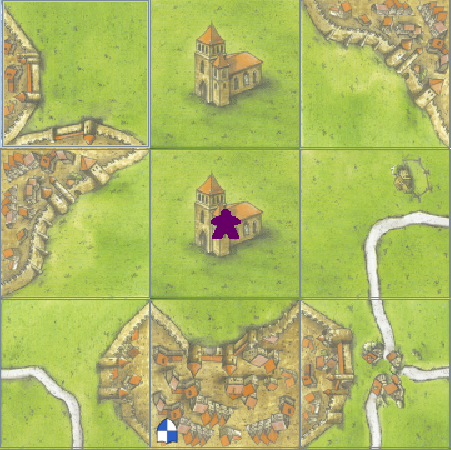
\includegraphics[]{images/MonasteroMeeple.png}}

    \caption{Chiudere un monastero comporta che questo sia circondato da 8 tessere, facendo guadagnare al proprietario 9 punti}
\end{figure}

\begin{figure}[hb]
    {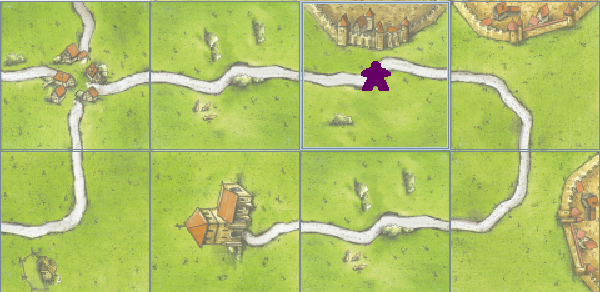
\includegraphics[]{images/StradaMeeple.png}}

    \caption{Chiudere una strada comporta la presenza di un incrocio o un’entrata ad un monastero/città da ambo i lati, facendo guadagnare al proprietario 1 punto per ogni tessera, estremi compresi}
\end{figure}

\begin{figure}[hb]
    %{\includegraphics[]{images/Prato.png}}

    \caption{Chiudere una prateria non fa guadagnare punti al proprietario, ma a fine partita esso otterrà 3 punti per ogni città chiusa confinante. Questo comporta che un seguace posizinato su una prateria non verrà mai ripreso dal giocatore fino a fine della partita}
\end{figure}

è possibile che due strutture in cui sono piazzati due o più seguaci (anche dello stesso colore) vengano unite tramite una tessera di congiunzione. In questo caso alla chiusura della struttura il giocatore che avrà la maggioranza di seguaci otterrà i punti vincendo su tutti gli altri. In caso di pareggio ogni giocatore otterrà la totalità dei punti.

Le difficoltà primarie sono:
\begin{itemize}
    \item rappresentare il concetto di tessera coerentemente con la sua rappresentazione grafica
    \item rappresentare il concetto di struttura
    \item unire strutture dello stesso tipo
    \item fare il conteggio dei punti rispettando le regole del gioco
\end{itemize}

